\documentclass[openright, a4paper]{article}
\usepackage{graphicx}
\usepackage{kotex}
\usepackage{minted}
\usepackage{setspace}
\usepackage{underscore}
\usepackage{caption}
\setminted{
    linenos=true,
    autogobble,
}
\newenvironment{longlisting}{\captionsetup{type=listing}}{}
\usepackage[margin=3cm]{geometry}
\newcommand{\code}[1]{\texttt{#1}}
\captionsetup{labelformat=empty,labelsep=none}

\title{2024학년도 컴퓨터구조 Lab Assignment \#3\\
        Multicycle CPU}

\author{김도영, 선민수}
\date{2024년 4월 16일}

\onehalfspacing
\begin{document}

\maketitle

\section{Introduction}
이 과제에서는 Verilog를 이용하여, 이전에 구현한 singlecycle CPU에서 발전한 
multicycle CPU를 만드는 것을 목적으로 한다. Multicycle CPU와 singlecycle CPU의 
가장 큰 차이점은 한 명령어를 실행하는 데 여러 cycle을 사용한다는 점이다. 
이러한 차이점 때문에, 한 명령어를 실행하는 데 한 clock cycle만을 이용하는 
singlecycle CPU에 비해 다음과 같은 장점이 있다.

\begin{itemize}
    \item 가장 느린 명령어의 실행 속도에 다른 명령어의 실행 속도를 맞출 필요가
    없으므로 전체적인 실행 속도가 빠르다.

    \item 하나의 자원(ALU, memory, register file... etc)을 여러 cycle에 나누어
    사용할 수 있으므로 singlecycle CPU의 중복된 부분을 제거할 수 있다.
\end{itemize}

\section{Design}
본 과제에서 구현한 multicycle CPU는 P\&H 4판 Ch 4.5.에서 설명하는 multicycle 
CPU를 기준으로 강의 교안의 설계를 일부 반영하여 구현하였다. 교과서에서는 JAL,
JALR, ECALL, BEQ를 제외한 나머지 Branch 명령어들을 구현하지 않았으며, 이러한 
부분들에 대하여 강의 교안의 설계를 반영하였다.

{
    \begin{figure}[!h]
        \centering
        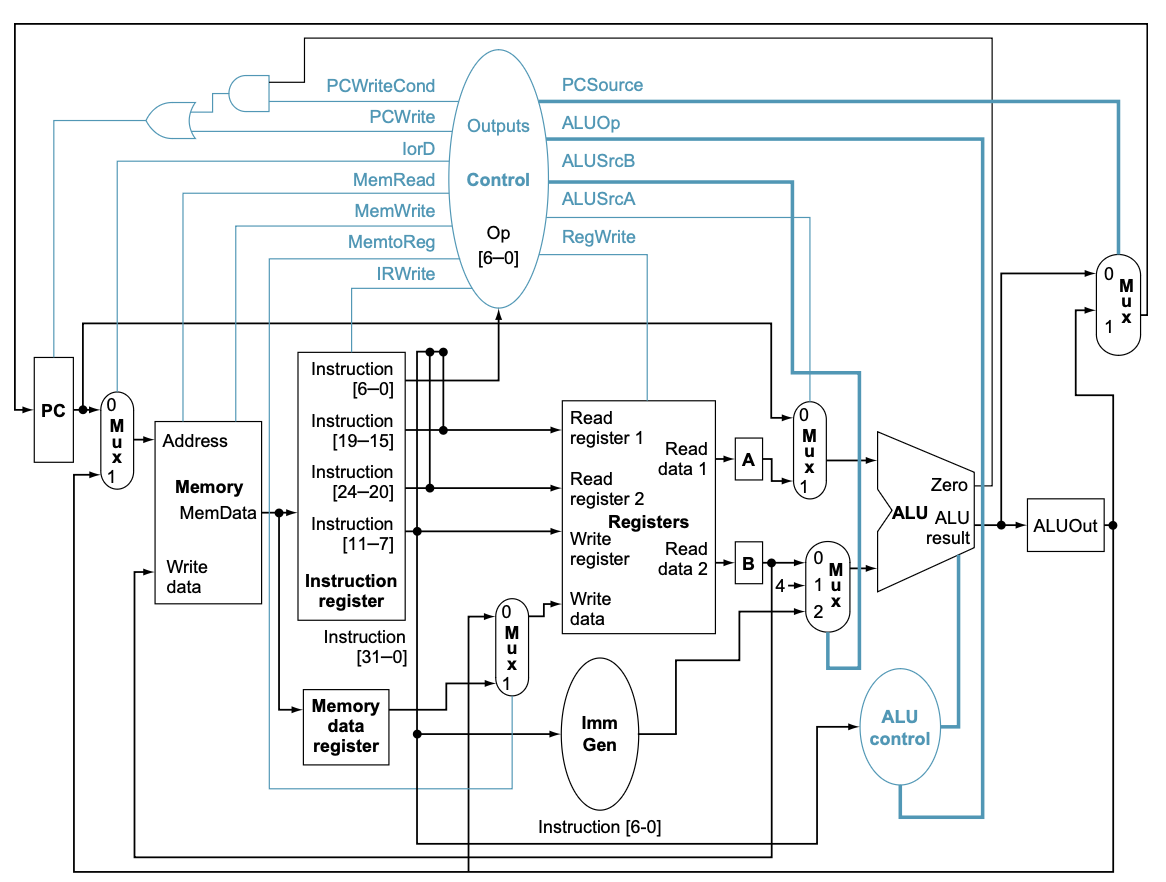
\includegraphics[width=\textwidth]{multicycle-module-diagram.png}
        \label{fig:design}
        \caption{Multicycle CPU의 전반적인 모듈 설계.}
    \end{figure}
}

Multicycle CPU를 구현하는데 쓰이는 각각의 세부 모듈과 그 구현은 다음과 같다.

\hfill

\begin{itemize}
    \item PC: 현재의 program counter 값을 저장하는 모듈로, clock의 positive 
    edge마다 \code{next_pc} 신호를 받아 \code{pc_update} 신호가 \code{1}일 때 
    program counter를 업데이트하는 동기 회로이다.

    \item Memory: 실제 CPU에 연결된 memory의 역할을 하는 모듈로, singlecycle 
    CPU의 구현과 다르게 명령어와 데이터를 모두 저장하며, clock의 positive 
    edge마다 입력에 따라 메모리 값을 변경하는 동기 회로이다.

    \item Instruction register: Memory에서 불러온 명령어를 해당 명령어가 
    실행되는 동안 저장해두는 레지스터로, clock의 positive edge에만 업데이트되는 
    동기 회로이다.

    \item Memory data register: Memory에서 불러온 데이터를 다음 명령어가 
    실행되기 전까지 저장해두는 레지스터로, clock의 positive edge에만 
    업데이트되는 동기 회로이다.

    \item Registers: CPU의 programmer visible state 중 하나인 레지스터이다. 
    \code{x0}부터 \code{x31}까지 총 32개를 가지고 있으며, clock의 positive 
    edge에만 업데이트되는 동기 회로이다.

    \item Control: 현재 명령어의 opcode를 받아 명령어의 실행 과정에 따라 
    해당하는 control 신호를 계산하는 모듈이다. 이때, singlecycle 구현과 다르게 
    여러 cycle에 걸쳐 다른 control 신호를 출력해야 하므로, clock의 positive 
    edge에만 업데이트되는 동기 회로로 구현되었다.

    \item A, B: 레지스터의 값을 다음 명령어의 instruction decode stage 전 까지 
    저장하는 레지스터로, clock에 맞추어 업데이트되는 동기 회로이다.

    \item ALU: 두 입력값과 ALU contorl 신호를 받아 해당하는 연산을 하는 
    모듈로, 입력이 바뀌면 출력도 곧바로 바뀌는 비동기 회로이다.

    \item ImmGen: 명령어를 받아 명령어에 따른 immediate 값을 계산하는 모듈로, 
    비동기 회로이다.

    \item ALU control: ALU가 수행해야 할 연산을 지정해주는 ALU control 신호를 
    계산하는 비동기 회로 모듈이다.

    \item ALUOut: ALU의 결과값을 다음 ALU 연산 전까지 저장해두는 레지스터로, 
    clock의 postivie edge에 맞추어 업데이트되는 동기 회로이다.
\end{itemize}

\hfill

Multicycle CPU는 한 명령어가 여러 clock cycle에 걸쳐서 실행될 수 있다. 따라서,
singlecycle CPU에서 \code{ControlUnit}이 현재 명령어에 의해서만 출력이 결정되는
조합 논리 회로였던 것과 달리, multicycle CPU의 \code{ControlUnit}은 내부 상태와
현재 입력에 따라서 출력이 결정되는 순차 논리 회로, 그 중에서도 유한 상태 기계로
구현된다.

\hfill

Multicycle CPU가 여러 clock cycle에 겹쳐서 실행될 수 있고, 각 모듈이 재사용되는 순간들이 있기 때문에, 유한 상태 기계를 보조하기 위해 사용되는 데이터들을 재사용할 필요가 있다.
이런 Resource Reuse는 다음과 같은 register로 구현되도록 하며 각 register의 값은 동기적으로 업데이트된다.
Instruction Register의 경우 MDR과 같이 Memory에서 fetch되므로, 이를 구분하기 위해 \code{ir_write} control signal을 이용해서 필요한 경우에만 업데이트한다.
(위에서 제시한 Multicycle CPU의 전반적인 모듈 설계 그림에서와 같은 이름을 사용한다.)

\begin{itemize}
    \item Instruction Register: FSM의 state에 의하여 현재가 아닌 추후에 결정되어야 하는 control signal을 위하여 fetch하였던 instruction을 instruction register에 저장한다.
    \item Memory Data Register(MDR): Memory에서 fetch하여 불러오는 데이터가 저장되는 register이다.
    \item A, B: Register File로부터 Register의 값이 Fetch된 결과를 저장하고 있는 Register이다.
    \item ALUOut: 이전에 연산되어있던 데이터를 재활용할 필요가 있는 경우(i.e. PC를 업데이트하는 경우) ALU의 결과 값이 저장되는 register이다.
\end{itemize}

\hfill

ControlUnit의 각 상태와 그에 따른 출력, 상태 전이를 명시한
다이어그램은 다음과 같다. 이때, 각 상태에 따른 출력이 명시되지 않은 신호들은
암묵적으로 \code{0}으로 간주하며, 출력의 이름이 명시되었으나 값이 명시되지 않은
신호들은 1-bit \code{1'b1}이다. 예를 들어, Instruction Decode stage에서
\code{alu_op}는 \code{2'b00}이며, Branch Computation stage에서 \code{pc_write}는
\code{1'b1}이다.

{
    \begin{figure}[!h]
        \centering
        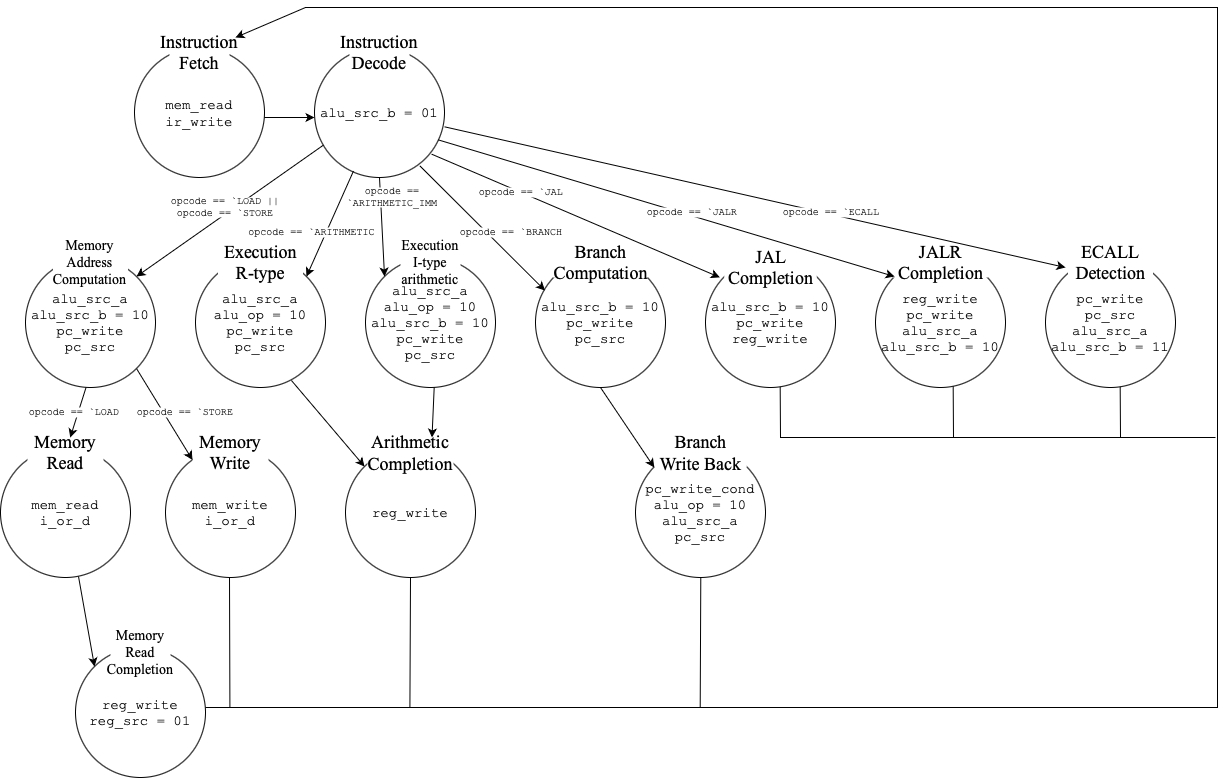
\includegraphics[width=\textwidth]{multicycle-fsm.png}
        \label{fig:design}
        \caption{ControlUnit 모듈의 FSM 다이어그램.}
    \end{figure}
}

\begin{itemize}
    \item Instruction Fetch state: Memory에서 명령어를 가져오는 stage이다.

    \item Instruction Decode stage: 명령어에 따라 해당하는 레지스터 값들을 A, B
    레지스터에 저장하는 stage이다. 이때, ALU에서 \code{PC + 4}값 또한 같이
    계산하여 ALUOut 레지스터에 저장한다.

    \item Memory Address Computation stage: LOAD, STORE 명령어를 실행하는데
    필요한 주소값을 계산하는 stage로, program counter 또한 동시에 ALUOut에 
    저장된 \code{PC + 4}로 업데이트한다.

    \item Execution R-type stage: R-type 산술 명령어를 실행하여 그 결과값을
    ALUOut에 저장하는 stage로, 위와 같이 PC 또한 업데이트한다.

    \item Execution I-type arithmetic stage: I-type 산술 명령어를 실행하여
    그 결과값을 ALUOut에 저장하는 stage로, 위와 같이 PC 또한 업데이트한다.

    \item Branch Computation stage: BRANCH 명령어의 결과 주소값을 계산하는
    stage로, 분기가 taken되지 않을 때를 대비하여 PC를 \code{PC + 4}로 
    업데이트한다.

    \item JAL Completion stage: JAL 명령어의 결과 주소값을 계산하고 이로 PC를 
    업데이트하며, \code{rd} 레지스터를 \code{PC + 4}로 업데이트하는 stage이다.

    \item JALR Completion stage: JALR 명령어의 결과 주소값을 계산하고 이로 PC를 
    업데이트하며, \code{rd} 레지스터를 \code{PC + 4}로 업데이트하는 stage이다.

    \item ECALL Detection stage: ECALL 명령어일 때 \code{GPR[x17]}의 값과 
    \code{10}을 비교하는 연산을 수행하는 stage이다.

    \item Memory Read stage: Memory Address Computation stage에서 계산한 주소를
    기반으로 memory 값을 읽어 이를 Memory Data Register에 저장하는 stage이다.

    \item Memory Write stage: Memory Address Computation stage에서 계산한 주소를
    기반으로 memory의 해당 주소에 B 레지스터의 값을 저장하는 stage이다.

    \item Arithmetic Completion: R-type, I-type 산술 연산의 결과를 레지스터에
    저장하는 stage이다.

    \item Branch Write Back stage: 분기 조건을 검사하여 만약 분기가 taken되었을
    경우 PC를 분기 목표 주소로 업데이트하는 stage이다.

    \item Memory Read Completion stage: Memory Read stage에서 저장한 memory 값을
    레지스터에 다시 저장하는 stage이다.

\end{itemize}

\section{Implementation}
ControlUnit과 ALUControl을 제외한 다른 모듈들은 singlecycle 구현과
대동소이하므로, 이 두 모듈의 구현에 집중하며, resource reuse를 위한 구현만을 추가적으로 설명한다.

\subsection{ControlUnit}
\begin{longlisting}
    \begin{minted}[fontsize=\footnotesize]{Verilog}
...
// Calculate the next state.
always @(*) begin
    case(state)
    `IF: next_state = `ID;

    `ID: begin
        case(opcode)
        `ARITHMETIC:     next_state = `EXR;
        `ARITHMETIC_IMM: next_state = `EXI;
        `LOAD:           next_state = `MAC;
        `JALR:           next_state = `JALRC;
        `STORE:          next_state = `MAC;
        `BRANCH:         next_state = `BC;
        `JAL:            next_state = `JALC;
        `ECALL:          next_state = `ED;
        default:         next_state = state;
        endcase
    end

    `MAC: begin
        if(opcode == `LOAD)
            next_state = `MR;
        else if(opcode == `STORE)
            next_state = `MW;
        else
            next_state = state;
    end

    `EXR:    next_state = `AC;
    `EXI:    next_state = `AC;
    `BC:     next_state = `BWB;
    `JALC:   next_state = `IF;
    `JALRC:  next_state = `IF;
    `MR:     next_state = `MRC;
    `MW:     next_state = `IF;
    `AC:     next_state = `IF;
    `MRC:    next_state = `IF;
    `ED:     next_state = `IF;
    `BWB:    next_state = `IF;
    default: next_state = state;
    endcase
end

// Compute output signal with respect to the current state.
always @(*) begin
    pc_write_cond = (state == `BWB);

    pc_write      = (state == `MAC)  || (state == `EXR)  || 
                    (state == `EXI)  || (state == `JALC) || 
                    (state == `JALRC) || (state == `BC) ||
                    (state == `ED);

    i_or_d        = (state == `MR) || (state == `MW);
    mem_read      = (state == `IF) || (state == `MR);
    mem_write     = (state == `MW);

    reg_src = (state == `MRC);
    ir_write = (state == `IF);

    pc_src = (state == `MAC) || (state == `EXR) || (state == `ED) ||
             (state == `EXI) || (state == `BWB) || (state == `BC);

    alu_op = {
        (state == `EXR) || (state == `EXI) || (state == `BWB) || (state == `ED),
        1'b0
    };

    alu_src_a = (state == `MAC) || (state == `EXR) || (state == `EXI) ||
                (state == `BWB) || (state == `JALRC) || (state == `ED);

    alu_src_b = {
        (state == `MAC) || (state == `EXI) || (state == `BC) || 
        (state == `JALC) || (state == `JALRC) || (state == `ED),
        (state == `ID) || (state == `ED)
    };

    reg_write = (state == `JALC) || (state == `JALRC) || (state == `AC) || (state == `MRC);
end
...
    \end{minted}
    \caption{ControlUnit.v}
\end{longlisting}
\break

ControlUnit은 CPU 전체의 control 신호를 출력하는 모듈로, 각 cycle에 따라 다른
신호를 내보내어 CPU를 구성하는 모듈이 cycle에 따라 다른 기능을 수행하도록 하고, 
때문에 하나의 자원을 재사용할 수 있도록 한다. 예를 들어, Instruction 
Decode에서는 \code{alu_src_b}를 \code{2'b01}로 설정하며 ALU가 \code{PC + 4}를
계산하도록 하는데, 이러한 ALU 출력은 ALUOut 레지스터에 저장되고, 이는 다시
Execution R-type과 같은 stage에서 \code{alu_op}를 \code{2'b10}으로 설정하여
ALU를 재사용할 수 있게 한다.

\subsection{ALUControl}
\begin{longlisting}
    \begin{minted}[fontsize=\footnotesize]{Verilog}
```
always @(*) begin
    case(aluOp)
        2'b00: alu_op_o = `ALU_ADD;
        2'b01: alu_op_o = `ALU_SUB;
        default: begin
            case(instruction[6:0])
                `ARITHMETIC: begin
                    case(instruction[14:12])
                        `FUNCT3_ADD: alu_op_o = (instruction[30]) ? `ALU_SUB : `ALU_ADD;
                        `FUNCT3_SLL: alu_op_o = `ALU_SLL;
                        `FUNCT3_SRL: alu_op_o = `ALU_SLR;
                        `FUNCT3_AND: alu_op_o = `ALU_AND;
                        `FUNCT3_OR:  alu_op_o = `ALU_OR;
                        `FUNCT3_XOR: alu_op_o = `ALU_XOR;
                        default: alu_op_o = 4'b0;
                    endcase
                end
                `ARITHMETIC_IMM: begin
                    case(instruction[14:12])
                        `FUNCT3_ADD: alu_op_o = `ALU_ADD;
                        `FUNCT3_SLL: alu_op_o = `ALU_SLL;
                        `FUNCT3_SRL: alu_op_o = `ALU_SLR;
                        `FUNCT3_AND: alu_op_o = `ALU_AND;
                        `FUNCT3_OR:  alu_op_o = `ALU_OR;
                        `FUNCT3_XOR: alu_op_o = `ALU_XOR;
                        default: alu_op_o = 4'b0;
                    endcase
                end
                `BRANCH: begin
                    case(instruction[14:12])
                        `FUNCT3_BEQ: alu_op_o = `ALU_BEQ;
                        `FUNCT3_BNE: alu_op_o = `ALU_BNE;
                        `FUNCT3_BLT: alu_op_o = `ALU_BLT;
                        `FUNCT3_BGE: alu_op_o = `ALU_BGE;
                        default: alu_op_o = 4'b0;
                    endcase
                end
                `LOAD: alu_op_o = `ALU_ADD;
                `STORE: alu_op_o = `ALU_ADD;
                `JAL: alu_op_o = `ALU_ADD;
                `JALR: alu_op_o = `ALU_ADD;
                `ECALL: alu_op_o = `ALU_BEQ;
                default: alu_op_o = 4'b0;
            endcase
        end
    endcase
end
```
    \end{minted}
    \caption{ALUControl.v}
\end{longlisting}

ALU에게 \code{alu_op_o}로 control signal을 넘겨주는 ALUControl은 주어진 \code{aluOp}에 따라서 필요한 control signal을 생성한다.
\code{2'b00}은 \code{ALU_ADD}를, \code{2'b01}은 \code{ALU_SUB}를 ALU에게 넘겨준다.
이외의 \code{aluOp}는 주어진 instruction의 FUCNT3, FUNCT7에 의해서 \code{alu_op_o}를 결정한다.
FUNCT7이 \code{ARITHMETIC}, \code{ARITHMETIC_IMM}, \code{BRANCH}인 경우에는 FUNCT3에 의해서 최종적인 \code{alu_op_o}가 결정된다.
이외의 FUNCT7에 경우에는 \code{ECALL}을 제외하고는 모두 ALU에서 ADD를 수행하기 때문에, \code{alu_op_o = `ALU_ADD'}로 넘겨준다.
\code{ECALL}의 경우에는 \code{cpu.v}에서 \code{is_halted} 조건을 검사할 때, ALU에 의한 bcond를 통해 x17 register의 값을 검사 하기 때문에, 이를 위해 \code{`ALU_BEQ'}를 통해서 조건 검사를 할 수 있도록 하였다.

\subsection{Resource Reuse}
\begin{longlisting}
    \begin{minted}[fontsize=\footnotesize]{Verilog}
```
    ...{전략}...

    reg [31:0] IR; // instruction register
    reg [31:0] MDR; // memory data register
    reg [31:0] A; // Read 1 data register
    reg [31:0] B; // Read 2 data register
    reg [31:0] ALUOut; // ALU output register

    always @(posedge clk) begin
        if(reset) begin
            IR <= 32'b0;
            MDR <= 32'b0;
            A <= 32'b0;
            B <= 32'b0;
            ALUOut <= 32'b0;
        end else begin
            if(ir_write)
                IR <= mem_dout;
            MDR <= mem_dout;
            A <= rs1_dout;
            B <= rs2_dout;
            ALUOut <= alu_result;
        end
    end

    ...{후략}...
```
    \end{minted}
    \caption{cpu.v}
\end{longlisting}

Design 섹션에서 설명하였듯이, 동기적으로 \code{clk} 신호에 맞추어 \code{IR}, \code{MDR}, \code{A}, \code{B}, \code{ALUOut}이 업데이트되는 것을 확인할 수 있다.
\code{IR}과 \code{MDR} 모두 \code{mem_dout에서} 값을 fetch하므로, \code{IR}은 control 신호 \code{ir_write}에 의해서만 업데이트 되는 것을 확인할 수 있다.

\section{Discussion}
\subsection{각 테스트벤치의 실행 cycle}

\begin{longlisting}
    \begin{minted}[fontsize=\footnotesize]{text}
### SIMULATING ###
TEST END
SIM TIME : 236
TOTAL CYCLE : 117 (Answer : 116)
FINAL REGISTER OUTPUT
 0 00000000
 1 00000000
 2 00002ffc
 3 00000000
 4 00000000
 5 00000000
 6 00000000
 7 00000000
 8 00000000
 9 00000000
10 00000013
11 00000003
12 ffffffd7
13 00000037
14 00000013
15 00000026
16 0000001e
17 0000000a
18 00000000
19 00000000
20 00000000
21 00000000
22 00000000
23 00000000
24 00000000
25 00000000
26 00000000
27 00000000
28 00000000
29 00000000
30 00000000
31 00000000
Correct output : 32/32
    \end{minted}
    \caption{basic_mem.txt 실행 결과}
\end{longlisting}

\hfill \break
\code{basic_mem.txt} 실행 결과는 다음과 같으며, 실행에 걸린 총 cycle 수는 
117 cycle이다.

\begin{longlisting}
    \begin{minted}[fontsize=\footnotesize]{text}
### SIMULATING ###
TEST END
SIM TIME : 1962
TOTAL CYCLE : 980 (Answer : 977)
FINAL REGISTER OUTPUT
 0 00000000
 1 00000000
 2 00002ffc
 3 00000000
 4 00000000
 5 00000000
 6 00000000
 7 00000000
 8 00000000
 9 00000000
10 00000000
11 00000000
12 00000000
13 00000000
14 0000000a
15 00000009
16 0000005a
17 0000000a
18 00000000
19 00000000
20 00000000
21 00000000
22 00000000
23 00000000
24 00000000
25 00000000
26 00000000
27 00000000
28 00000000
29 00000000
30 00000000
31 00000000
Correct output : 32/32
    \end{minted}
    \caption{loop_mem.txt 실행 결과}
\end{longlisting}

\hfill \break
\code{loop_mem.txt} 실행 결과는 다음과 같으며, 실행에 걸린 총 cycle 수는 980
cycle이다.

\section{Conclusion}

이번에는 지난 Single Cycle CPU에서 발전한 Multi Cycle CPU를 구현하였다.
Single Cycle과는 달리 스테이지별로 필요한 clock만큼만 소요하여, Single Cycle CPU처럼 가장 실행이 오래 걸리는 instruction에 맞춘 clock speed를 가지지 않는다는 점이 특징이다.
Multi Cycle CPU는 Single Cycle CPU에서 FSM을 통한 flow control을 통하여 구현할 수 있었으며, total cycle에서는 증가할 수 있지만, clock frequency의 증가로 인해 결국 기존 Single Cycle CPU에서 발전한 것을 확인할 수 있었다.
다만 Multi Cycle CPU 또한 Single Cycle CPU에서 거론되었던, 기존 instruction이 수행되는 동안 사용되지 않는 stage의 모듈들이 모두 낭비되고 있는 점을 보완하지는 못하였고, 궁극적으로 이를 개선할 수 있는 Pipelined CPU의 필요성을 확인할 수 있었다.

\end{document}